\chapter{Despliegue y pruebas}
\label{chap:despliegue}

\textcolor{red}{En este capítulo describiremos cómo se llevó a acabo el despliegue de la solución y las pruebas que se realizaron.}

\section{Despliegue}

Debido a la gran cantidad de microservicios que componen la solución, desde muy temprano fue necesario definir un plan de despliegue. Su número iba en aumento y era muy complicado gestionarlos a mano. Para ello, optamos entonces por empaquetarlos en contenedores de \texttt{Docker}\footnote{Página oficial: \url{https://www.docker.com/}}. Gracias a esto podíamos iniciarlos y pararlos fácilmente. Además que nos aporta una serie de ventajas interesantes: ejecución aislada de los procesos, gestión más fácil de las dependencias, entre otras. \cite{newmanBuildingMicroservicesDesigning2021,delatorreNETMicroservicesArchitecture2021}

\begin{wrapfigure}{r}{0.23\linewidth}
  \vspace{-25pt}
  \centering
  
\includegraphics[scale=0.95]{cap_despliegue/images/docker-compose-logo}
  \vspace{-15pt}
\end{wrapfigure}

Para orquestar el despliegue de la solución optamos por \texttt{Docker Compose}\footnote{Página oficial: \url{https://docs.docker.com/compose/}}. Nos permite declarar la configuración del despliegue de nuestros servicios. Esto incluye los parámetros de ejecución, número de instancias, políticas de reinicio, etc. Aunque el bucle MAPE-K \foreign{english}{Lite} original corre sobre Kubernetes, no necesitábamos un orquestador tan ''pesado''. Nuestro plan era ejecutar la solución en un único \foreign{english}{host}.

\texttt{Docker Compose} también nos permite declarar las dependencias entre servicios. Esto fue clave para el despliegue del contenedor de \texttt{RabbitMQ}. Debido a que el protocolo requiere de una conexión permanente al bus\cite{johanssonPartRabbitMQBest2019}, todos los servicios que dependen de él deben desplegarse después. Por ello, declaramos una dependencia con este servicio y definimos una política de reintentos.

\subsection{Observabilidad y telemetría}

Un punto en el que queremos hacer hincapié es en la telemetría. Debido a que estamos tratando con un sistema distribuido, es complicado conocer su estado global en un momento determinado. Especialmente en este caso, en el que participan más de diez microservicios distintos. Si necesitáramos depurar y diagnosticar el comportamiento del sistema, es muy difícil trazar el impacto de una petición.

Por defecto, solo contábamos con los \emph{logs} (registros), que mostramos en la figura \ref{fig:console-logs}. Aparecen intercalados en una única ventana los de todos los servicios y peticiones concurrentes. Aunque nos pueden resultar utilidad, es una aproximación ineficiente. Incluyen demasiada información y es difícil de procesar para una persona. Además que, según aumente la carga de peticiones, aumentará el número de registros y se volverá más difícil de interpretar.

\begin{figure}[h]
  \centering
  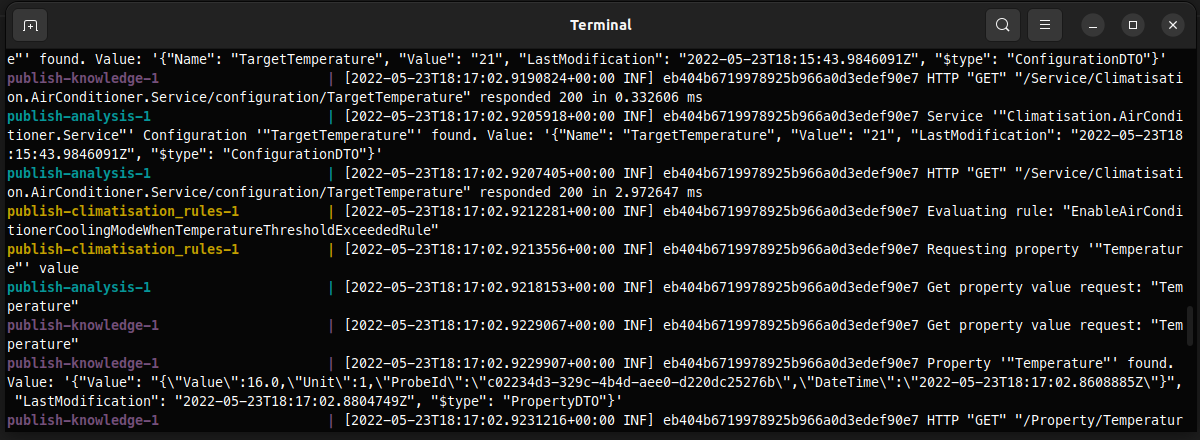
\includegraphics[scale=1.45]{cap_despliegue/images/console-logs}
  \caption{Extracto de \emph{logs} de una ejecución habitual.}
  \label{fig:console-logs}
\end{figure}

En el ámbito de los sistemas distribuidos requerimos de soluciones de monitorización y \foreign{english}{logging} más avanzadas. \cite{newmanBuildingMicroservicesDesigning2021} Nuestros servicios tendrán que recopilar y reportar datos de su funcionamiento, lo que se conoce como \textbf{telemetría}. Esto requerirá de \textbf{instrumentar} nuestros sistemas con distintas herramientas o \textbf{sondas}. Es exactamente lo mismo que hacemos en la etapa de monitorización del bucle MAPE-K.

Para explotar estos datos recurrimos a técnicas de \textbf{observabilidad}. Según \cite{parkerProblemDistributedTracing2020}, la observabilidad <<\emph{no es sólo un método para monitorizar sistemas en producción, si no también para ser capaces de entender su comportamiento usando un número relativamente bajo de señales}>>. Con \textbf{señales} se refiere a las distintas fuentes de información de telemetría de las que dispongamos.

La observabilidad nos ayuda a detectar \textbf{fluctuaciones en el funcionamiento} de nuestro sistema. Estas puedes ser errores, realentizaciones, caídas de servicios, etc. También nos permite \textbf{explicar sus causas} a partir de las señales. De nuestros servicios podemos capturar tres tipos de señales distintos. Todas ellas son complementarias, ya que reflejan el funcionamiento desde distintas perspectivas. Son conocidas como \textbf{los tres pilares de la observabilidad}:

\begin{itemize}
  \item \textbf{\foreign{english}{Logs}}: Se trata de eventos de la aplicación que se registran durante su funcionamiento. Pueden ser simples cadenas de texto o estructuras de datos más complejas. En el segundo caso, se trata de registros enriquecidos con propiedades que les dotan de más contexto. Es el mecanismo de telemetría que ofrece más detalle del funcionamiento de un servicio concreto. También es el más usado.

  \item \textbf{Métricas}: Son datos agregados que nos permiten conocer el estado global de nuestros servicios. \cite{opentelemetryOpenTelemetryDocumentation2022} Se calculan a partir de mediciones de parámetros del servicio en un momento determinado. Por ejemplo del número de peticiones recibidas, su duración, etc. Normalmente se representan cómo series temporales: peticiones por segundo, duración media de las peticiones, etc.

  \item \textbf{Trazas distribuidas}: Se trata del mecanismo más reciente. Es una forma de registrar el recorrido que hace una petición a través de los distintos microservicios que componen nuestro sistema. Nos permite ver cómo participa cada uno de ellos en la operación y qué impacto tiene en el rendimiento. \cite{parkerProblemDistributedTracing2020}

  Para registrar una traza, le asignaremos a la petición un identificador único que se propagará con cada sub-petición. Están compuestas por \foreign{english}{spans}, operaciones que se realizan dentro de la petición. Cada uno puede tener otras sub-operaciones anidadas. \cite{opentelemetryOpenTelemetryDocumentation2022}
\end{itemize}

Para explotar estos datos, necesitaremos entonces poder hacer consultas sobre ellos. Pongamos por ejemplo que hemos detectado que ha aumentado considerablemente la métrica de la duración media de las peticiones. A partir de la fecha y hora de este suceso, deberíamos poder recuperar la información necesaria para responder a la pregunta de qué ha pasado. Ya sean \foreign{english}{logs}, trazas u otras métricas relacionadas.

Con este fin se surgen las \textbf{plataformas de observabilidad}. Se trata de conjuntos de servicios que capturan los datos de telemetría. Los procesan y almacenan para su posterior consulta. También contamos con servicios que nos permiten visualizar y consultar de forma conjunta toda esta información. Por ejemplo, mediante \foreign{english}{dashboards} o paneles.

\subsubsection{Plataforma de observabilidad}

Para poder capturar y explotar estas señales, necesitaremos construir nuestra propia plataforma de observabilidad. Para este trabajo hemos optado por una combinación de cuatro servicios. \texttt{Grafana Loki} para capturar los \foreign{english}{logs}. \texttt{Prometheus} para capturar las métricas. \texttt{Jaeger} para capturar las trazas distribuidas. Y \texttt{Grafana} para visualizar y consultar todos los datos.

\begin{wrapfigure}{r}{0.15\linewidth}
  \vspace{-10pt}
  \hspace{10pt}
  \centering
  
\includegraphics[scale=0.5]{cap_despliegue/images/opentelemetry-logo}
\end{wrapfigure}

Para capturar la telemetría, empleamos el estándar \textbf{OpenTelemetry}\footnote{Página oficial: \url{https://opentelemetry.io/}}. Se trata de un proyecto desarrollado por la Cloud Native Computing Foundation (CNCF). Tiene el objetivo de definir un mecanismo estándar para recopilar y transmitir datos de telemetría. Para ello, ofrece un conjunto de librerias que nos permite instrumentar nuestras aplicaciones. Podremos enviar estos datos a cualquier plataforma que ofrezca extensiones compatibles.

Con estas herramientas hemos instrumentado todos nuestros servicios. Nuestra plataforma de observabilidad tiene la siguiente estructura (figura \ref{fig:observability-telemetry-collection}):

\begin{figure}[h!]
  \centering
  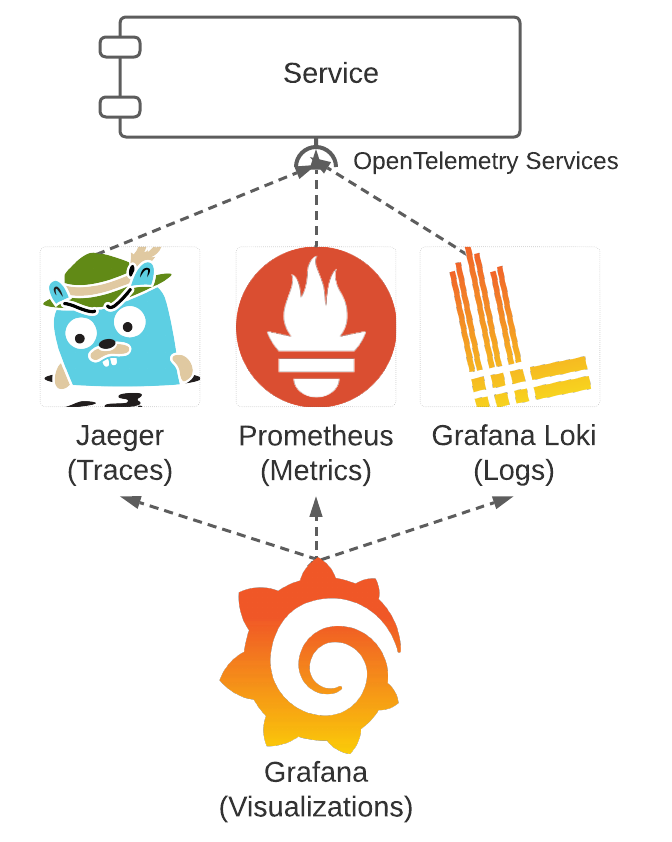
\includegraphics[scale=0.28]{cap_despliegue/images/observability-telemetry-collection}
  \caption{Estructura de nuestra plataforma de observabilidad}
  \label{fig:observability-telemetry-collection}
\end{figure}

\subsubsection{Grafana Loki: \foreign{english}{Logs}}

\begin{wrapfigure}{r}{0.10\linewidth}
  \vspace{-7pt}
  \hspace{-10pt}
  \centering
  
\includegraphics[scale=0.85]{cap_despliegue/images/Loki}
\end{wrapfigure}

\texttt{Loki}\footnote{Página oficial: \url{https://grafana.com/oss/loki/}} es un agregador de \foreign{english}{logs} estructurados desarrollado por Grafana Labs. Todos los servicios instrumentados se los enviarán y este los almacenará de forma centralizada. Para facilitar las consultas, Loki indexa todos los registros en base a etiquetas (\foreign{english}{labels}), metadatos especificados por el usuario. Por ejemplo, el nivel (información, \foreign{english}{warning}...) o el nombre del servicio que los emite.

Nuestros servicios emiten los \foreign{english}{logs} siguiendo el mismo convenio. Estos deben incluir la fecha del evento y su nivel de severidad. También incluirán propiedades que indiquen el nombre del emisor y el del entorno en el que se encuentra. Además, queremos correlacionar \foreign{english}{logs} de distintos servicios que se originen de una misma petición. Para ello los etiquetaremos con un identificador único: el identificador de la traza (\texttt{traceId}). En la figura \ref{fig:loki-ejemplo-logs} mostramos un ejemplo de toda la información registrada.

\begin{figure}[h]
  \centering
  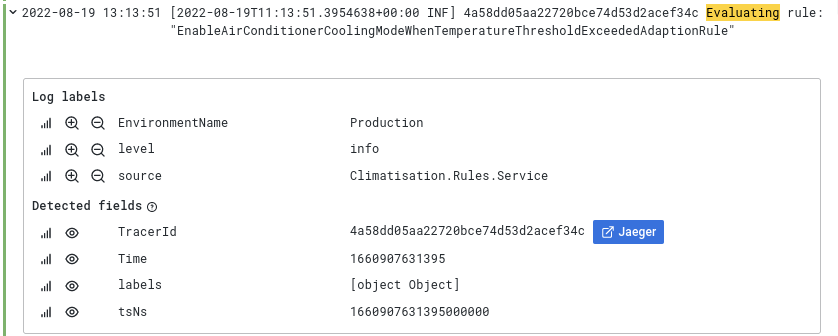
\includegraphics[scale=0.5]{cap_despliegue/images/Ejemplo-log}
  \caption{Ejemplo de la estructura de un registro.}
  \label{fig:loki-ejemplo-logs}
\end{figure}

\subsubsection{Prometheus: Métricas}

\begin{wrapfigure}{r}{0.10\linewidth}
  \vspace{-12pt}
  \centering
  
\includegraphics[scale=0.025]{cap_despliegue/images/prometheus-logo}
\end{wrapfigure}

\texttt{Prometheus}\footnote{Página oficial: \url{https://prometheus.io/}} es una herramienta de monitorización y alertas desarrollada originalmente por SoundCloud. Nos permite capturar mediciones de parámetros de nuestros servicios. Estas serán procesadas y almacenadas como series temporales. Sobre ellas, podremos hacer distintos tipos de análisis, consultas y visualizaciones.

Por defecto, ASP.NET captura distintas métricas que podemos exponer con Prometheus. También nos permite definir las nuestras propias. Estas pueden ser de distintos tipos. Los más habituales son los \textbf{contadores} e \textbf{indicadores}. \cite{parkerProblemDistributedTracing2020} Los primeros aumentan su valor cada vez que ocurre un evento determinado. Por ejemplo, el número de peticiones recibidas. Por otro lado, los indicadores representan un valor en un momento determinado. Por ejemplo, el número de usuarios activos actualmente.

Para importar los datos, el servidor de Prometheus ejecutará periódicamente consultas HTTP sobre un \foreign{english}{endpoint} estándar: \texttt{GET /metrics}. Nuestros servicios instrumentados expondrán sus métricas y mediciones allí. En la figura \ref{fig:prometheus-ejemplo-metricas} tenemos un ejemplo. Muestra las métricas por defecto y algunas definidas por nosotros, como un contador de peticiones de configuraciones.

\begin{figure}[htb]
  \centering
  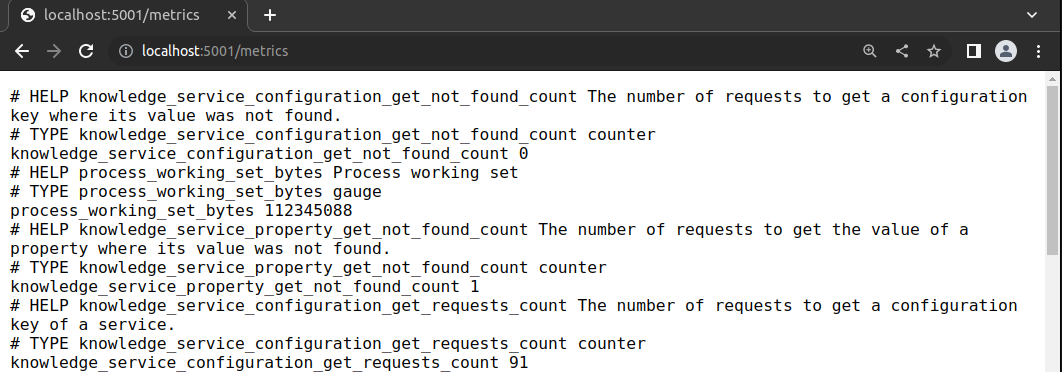
\includegraphics[scale=1.65]{cap_despliegue/images/Prometheus-Metricas-Ejemplo}
  \caption{Ejemplo de las métricas que expone el \foreign{english}{endpoint} de Prometheus en el servicio de conocimiento.}
  \label{fig:prometheus-ejemplo-metricas}
\end{figure}

\subsubsection{Jaeger: Trazas distribuidas}

\begin{wrapfigure}{r}{0.15\linewidth}
  \vspace{-20pt}
  
\includegraphics[scale=0.12]{cap_despliegue/images/jaeger-logo-x}
  \vspace{-20pt}
\end{wrapfigure}

Jaeger\footnote{Página oficial: \url{https://www.jaegertracing.io}} es un sistema para la captura de trazas distribuidas. Fue desarrollado originalmente por Uber Technologies. Todos los servicios instrumentados enviarán allí los fragmentos correspondientes a las actividades en las que participan (los \foreign{english}{spans}). A partir de ellas y el identificador común de la traza, es capaz de reconstruir la traza completa de la petición.

Gracias a las trazas distribuidas, podemos ver todas las actividades que desencadenó una petición concreta. Podemos ver sus nombres, su duración e incluso las sub-actividades en las que derivan. En nuestro caso, mostramos en la figura \ref{fig:jaeger-traza-distribuida} un fragmento de la traza del reporte de una medición de temperatura. Vemos que esta inicia con la actividad de reporte y que acaba desencadenando actividades en seis servicios distintos.

\begin{figure}[htb]
  \centering
  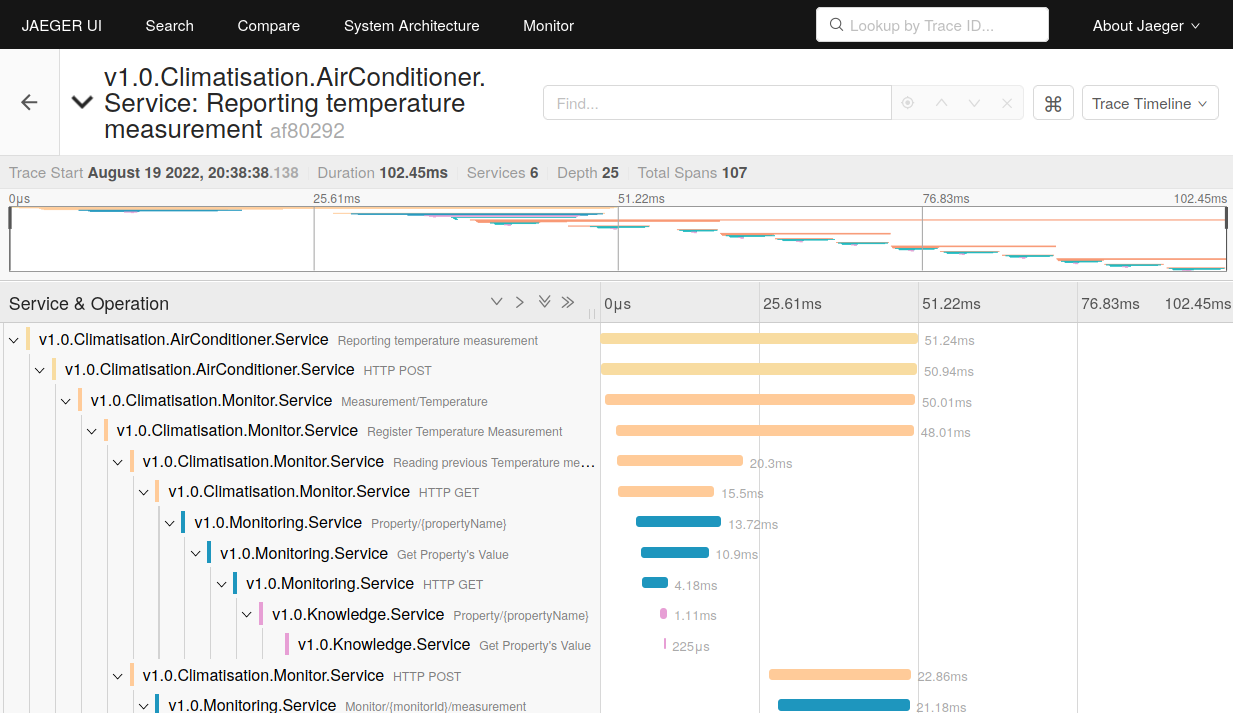
\includegraphics[scale=0.35]{cap_despliegue/images/jaeger-traza-distribuida}
  \caption{Ejemplo de una traza distribuida de Jaeger. Representa las actividades que desencadena el reporte de una medición de tempertura.}
  \label{fig:jaeger-traza-distribuida}
\end{figure}

A partir de las trazas, Jaeger también es capaz de inferir la arquitectura de nuestra aplicación. En la figura \ref{fig:jaeger-arquitectura-inferida} mostramos la arquitectura inferida de nuestro sistema de climatización. Podemos comprobar que la implementación respeta la jerarquía de los microservicios definida en este trabajo. Aunque, este diagrama no muestra el mecanismo de comunicación usado entre cada uno.

\begin{figure}[htb]
  \hspace{1.25cm}
  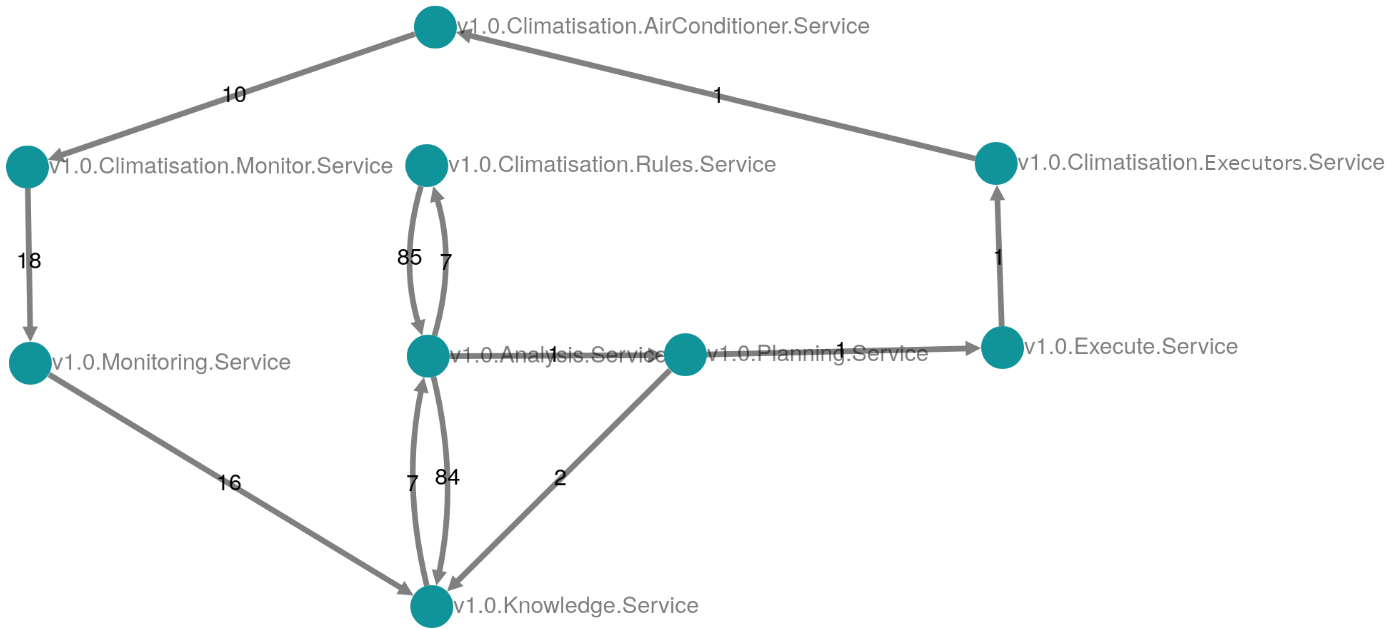
\includegraphics[scale=0.3]{cap_despliegue/images/Jaeger-arquitectura-climatizacion}
  \caption{Arquitectura inferida por Jaeger de nuestro sistema de climatización a partir de las trazas capaturadas.}
  \label{fig:jaeger-arquitectura-inferida}
\end{figure}

\subsubsection{Grafana: Visualización}

\begin{wrapfigure}{r}{0.15\linewidth}
  \vspace{-20pt}
  
\includegraphics[scale=0.10]{cap_despliegue/images/Grafana_logo}
  \vspace{-20pt}
\end{wrapfigure}

La última pieza del puzzle de observabilidad es Grafana. Desarrollado también por Grafana Labs, es una herramienta para la monitorización y visualización de datos. Gracias a su sistema de \foreign{english}{plugins}, es compatible con una gran variedad de fuentes de información: bases de datos, servicios web, servicios de métricas, etc.

Nos permite \textbf{explorar los datos} a través de consultas sobre las fuentes de información. Todas ellas se hacen usando los mecanismos ofrecidos por cada plataforma. Este sería el caso de Prometheus, donde podemos usar su lenguaje de consultas \texttt{PromQL}. Con él, podremos consultar y visualizar métricas. Esto nos permitirá explotar al máximo las capacidades de cada una.

Incluso, podemos ir más allá y \textbf{definir relaciones entre datos de fuentes distintas}. Retrocedamos a la figura \ref{fig:loki-ejemplo-logs}, que representa los \foreign{english}{logs} de Loki. Si nos fijamos, en el campo \texttt{TracerId} aparece un enlace a Jaeger. Al hacer clic en él, se desplegará en un panel lateral la traza de la petición a la que pertenece el registro. Todo esto nos será de gran ayuda a la hora de \textbf{investigar} los motivos de las fluctuaciones en el funcionamiento.

También se pueden aprovechar las consultas de las fuentes de datos para crear \textbf{paneles de monitorización}. Esto nos permitirá agregar en solo lugar a los \foreign{english}{logs}, las métricas y las trazas. A partir de ellos podemos crear todo tipo de visualizaciones útiles. Por ejemplo, del estado de las peticiones concurrentes, del número de errores, etc. En la figura \ref{fig:grafana-panel-monitorizacion} enseñamos nuestro panel de monitorización. Este nos muestra parámetros como la temperatura actual de la habitación (gráfica superior izquierda), un listado de las adaptaciones ejecutadas (panel de \foreign{english}{logs} bajo las temperaturas) o información técnica de los servicios (consumo de RAM, tiempo de CPU...). En la siguiente sección las explicaremos en más detalle.

\begin{landscape}

  \begin{figure}[htb]
    \centering
    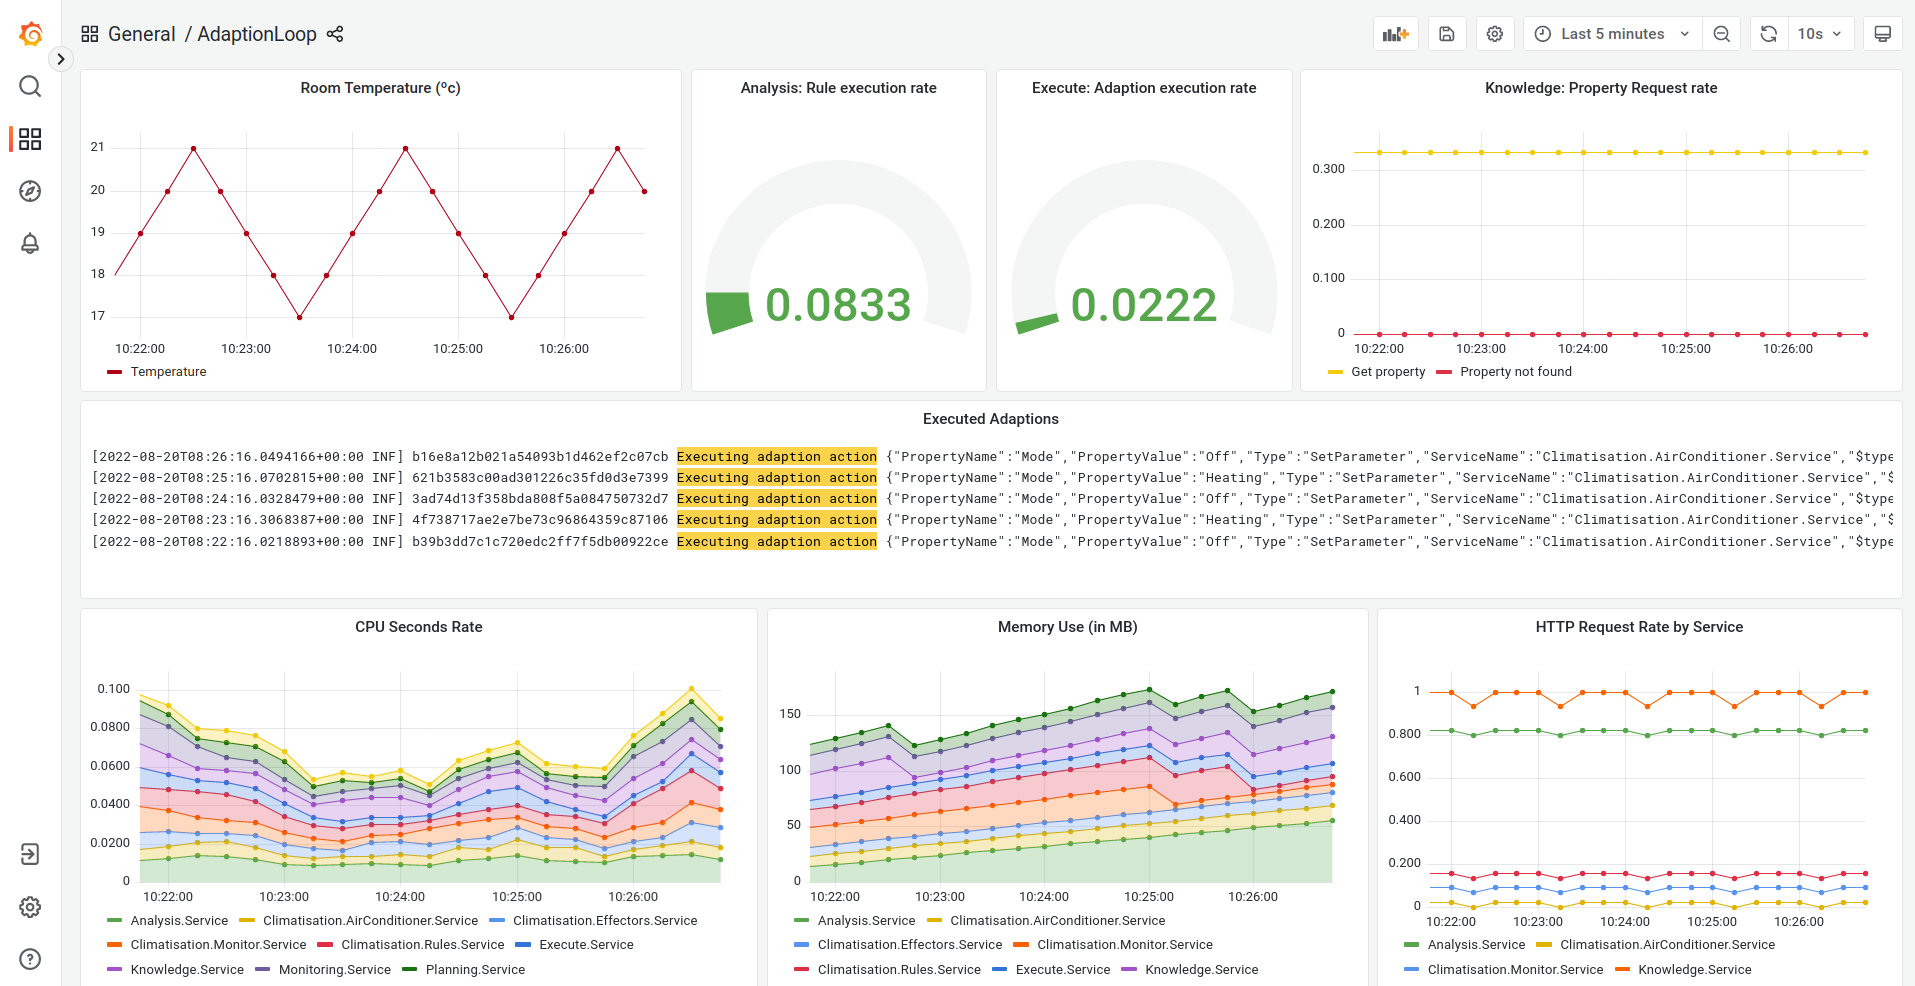
\includegraphics[scale=0.37]{cap_despliegue/images/Grafana-panel-monitorizacion}
    \caption{Panel de monitorización para la solución autoadaptativa de climatización.}
    \label{fig:grafana-panel-monitorizacion}
  \end{figure}

\end{landscape}


\section{Pruebas}

Finalmente, llegó el momento de poner a prueba nuestro sistema. Queríamos determinar si la arquitectura diseñada era viable o requería de algún refinamiento. Recordemos que el objetivo es aplicarla en el bucle MAPE-K \foreign{english}{Lite} original mediante una refactorización. Con esto en mente, diseñamos distintas pruebas para verificar su funcionamiento. Nos resultó de gran ayuda nuestra plataforma de observabilidad, que nos permitirá investigar distintas áreas de la solución.

Las primeras pruebas que ejecutamos fueron las relacionadas con el funcionamiento del sistema de climatización. Hasta que este no se estabilizará, no podíamos emitir ningún juicio sobre la arquitectura. En estos tests verificamos que, a partir de las mediciones de temperatura, debe ser capaz de completar el proceso de adaptación. Esto implica que todas las etapas del bucle MAPE-K se ejecutan correctamente. También incluimos pruebas de carga para analizar cómo se comportaba en situaciones extremas.

Completadas estas pruebas pasamos a verificar, ahora sí, aspectos de la arquitectura. Gracias a la telemetría que capturamos, pudimos responder a distintas preguntas sobre ella. Por ejemplo, si es correcta la división funcional que hemos elegido o si los mecanismos de comunicación son los adecuados. En base a las respuestas, pautamos una serie de correcciones que se podrían aplicar.

\subsection{Pruebas sobre el sistema de climatización}

\begin{wrapfigure}{r}{0.38\linewidth}
  \vspace{-15pt}
  \centering
  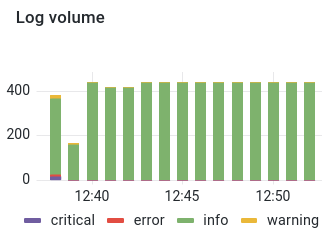
\includegraphics[scale=0.50]{cap_despliegue/images/pruebas-logs-error}
  \caption{Niveles de los \foreign{english}{logs} registrados durante la inicialización del sistema.}
  \label{fig:pruebas-logs-inicializacion}
  \vspace{-15pt}
\end{wrapfigure}

La primera prueba del sistema de climatización consistió en comprobar su \textbf{correcto despliegue}. Para ello, verificamos que después de este, todos los servicios estén operativos. También analizamos los \foreign{english}{logs} en busca de registros de error. Detectamos que durante la inicialización aparecen algunos (primera barra en la figura \ref{fig:pruebas-logs-inicializacion}). Una vez que se completa, el sistema se estabiliza y estos errores desaparecen (resto de barras). Todos provenían de servicios que dependen del \foreign{english}{broker} de mensajería (figura \ref{fig:prueba-logs-error-rabbitmq}). Como deben establecer una conexión con él durante el arranque, si no ha completado su despliegue todavía, fallarán.

Según el desarrollador de Rebus, estos errores podrían solucionarse implementado un \textbf{servicio en segundo plano que gestione la conexión}.\footnote{\url{https://github.com/rebus-org/Rebus.ServiceProvider\#delayed-start-of-the-bus}} De esta forma, el servicio no fallará durante el arranque e intentará periódicamente conectarse con RabbitMQ. Debido a restricciones de tiempo, en lugar de implementarlo así, optamos por definir una estrategia de reintentos en el fichero de Docker Compose. Así, los afectados se reiniciarán hasta que puedan establecer la conexión correctamente.

\begin{figure}[htb]
  \centering
  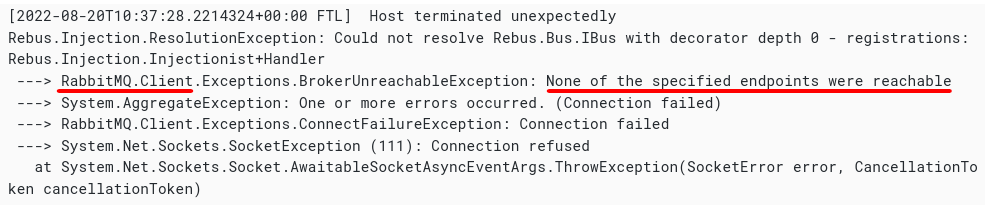
\includegraphics[scale=0.45]{cap_despliegue/images/Logs-fallo-RabbitMQ}
  \caption{Ejemplo de registro relacionado con el fallo al contactar con RabbitMQ durante el arranque.}
  \label{fig:prueba-logs-error-rabbitmq}
\end{figure}

A continuación, procedimos a realizar \textbf{pruebas sobre la funcionalidad}. En estas, nos centramos en verificar que el sistema \textbf{regula correctamente la temperatura} de la habitación. Recordemos que el servicio de aire acondicionado cuenta con un termómetro simulado. Cada 15 segundos, este reporta una medición de temperatura ficticia al monitor de climatización. Esta variará dependiendo del modo activo del aire acondicionado. En base a la temperatura, el bucle evaluará las reglas y pautará adaptaciones si lo considera necesario.

\textcolor{red}{Para ello, comprobaremos que se aplican las cuatro reglas definidas en la tabla \ref{tab:adaption-rules-climatisation}. Todas ellas activan o desactivan un modo del aire acondicionado cuando la temperatura alcanza un determinado umbral. Por ejemplo, si es muy alta, se debería activar el modo de refrigeración. Cuando se alcance la temperatura de confort, otra regla lo apagará.}

\textcolor{red}{Tenemos varias formas de verificarlo. La primera de ellas es mediante la visualización de la temperatura de nuestro panel de monitorización. En la figura \ref{fig:pruebas-temperatura} mostramos la aplicación de las cuatro reglas. A la derecha se muestran las dos reglas que acabamos de describir.}

\begin{figure}[h]
  \hspace{-1.2cm}
  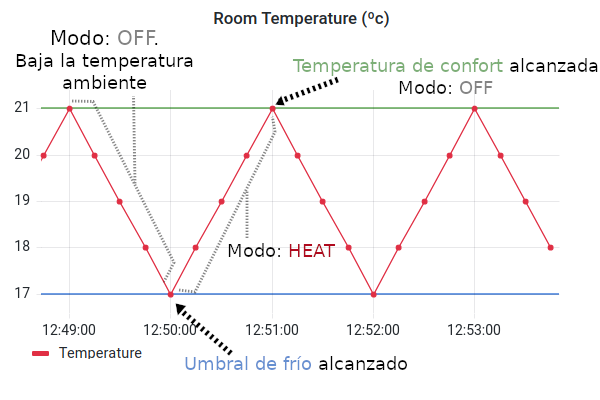
\includegraphics[scale=0.42]{cap_despliegue/images/pruebas-temperatura-calentar}
  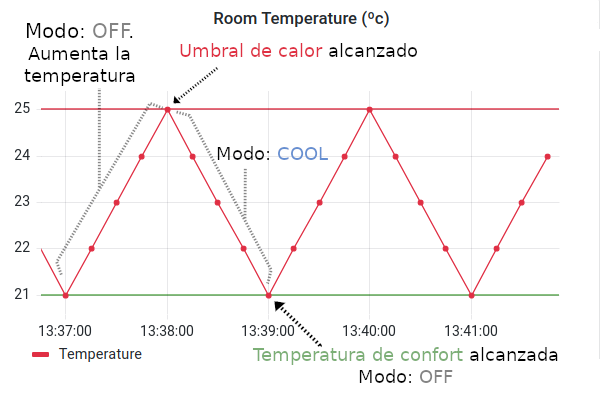
\includegraphics[scale=0.42]{cap_despliegue/images/pruebas-temperatura-enfriar}
  \caption{Gráficas extraídas de Grafana que muestran el funcionamiento de las adaptaciones. Izq.: Encender y apagar la calefacción. Der.: Encender y apagar la refrigeración.}
  \label{fig:pruebas-temperatura}
\end{figure}


Tenemos varias formas para comprobar si esto es así. La primera de ellas es la más evidente, mirando el

También comprobamos que las trazas pasen por todos las etapas correspondientes.


También probamos a asignar temperaturas manualmente a través de un endpoint. Así podíamos forzar manualmente a que se apliquen las reglas.

También podemos comprobar los logs para ver que se están aplicando las adaptaciones pertinentes cuando corresponde.


Otro tipo de prueba que implementamos fueron las de carga. Para ello, intentamos saturar el sistema mediante mediciones falsas de temperatura, para ver cómo reaccionara. Para ello, usamos la librería NBomber\footnote{Página oficial: \url{https://github.com/PragmaticFlow/NBomber}.}. Cuyo uso es justamente este.Con ella, pudimos ver que el

\subsection{Verificación de la arquitectura}

Una vez verificado el correcto funcionamiento del sistema, podemos proceder a verificar la arquitectura. Nos centraremos especialmente en los puntos en los que tenga lugar el mayor número de comunicación entre servicios.

Recuperando la figura \ref{fig:jaeger-arquitectura-inferida}, en ella se describe el resultado de reportar 10 mediciones de temperatura. De ellas, solo 1 medición ha provocado la adaptación del sistema. En ella, podemos comprobar que dos servicios están muy acoplados. El de reglas y el de análisis. Aparecen 85 peticiones síncronas desde las reglas al módulo de análisis. Esto nos indica que están muy acoplados \cite{singjaiPatternsDerivingAPIs2021}. Esto nos plantea que existen dos

Por otro lado, vemos también la misma dependencia entre el servicio de análisis y el conocimiento. EN este caso, la división funcional si que es clara. AParte de que el cocnocimiento está compartido entre distintos servicios del nivel del bucle. Por tanto, una mejor solución sería optimizar esta comunicación. Podríamos agrupar en una misma petición la solicitud de varias propiedades del conocimiento a la vez.

\begin{figure}[htb]
  \hspace{1.25cm}
  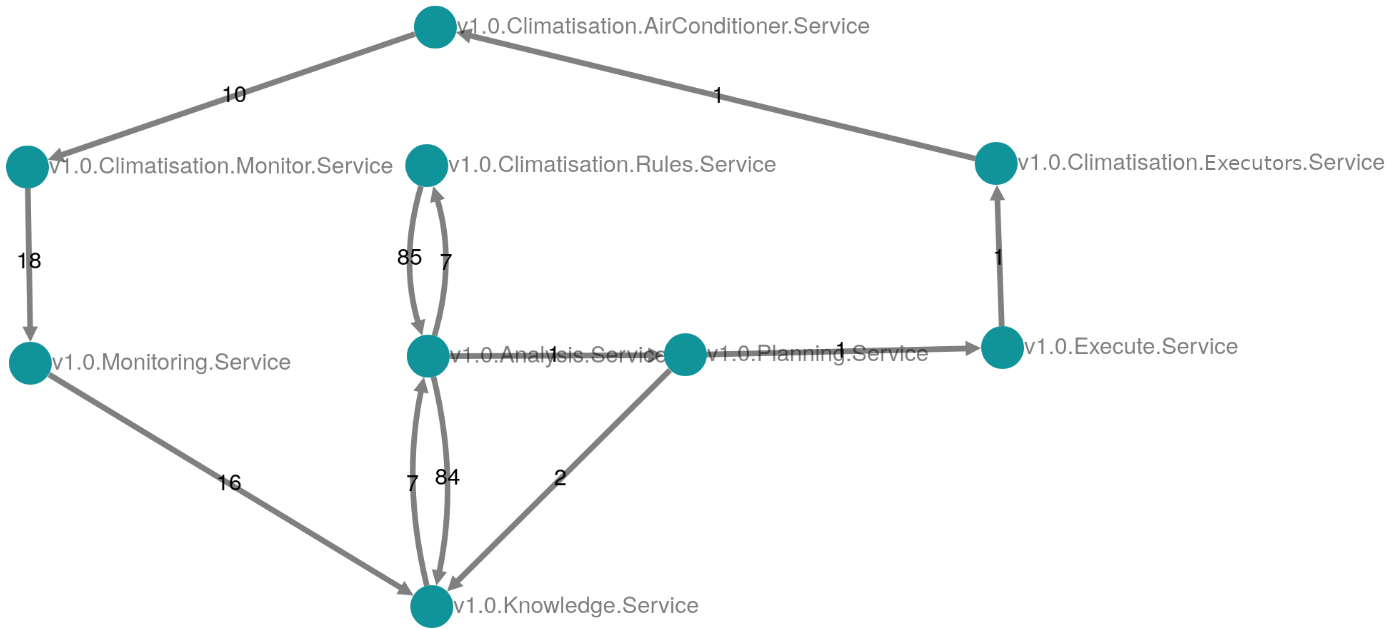
\includegraphics[scale=0.3]{cap_despliegue/images/Jaeger-arquitectura-climatizacion}
  \caption{Jaeger nos genera un esquema de la arquitectura de nuestra aplicación. Este muestra las comunicaciones entre servicios.}
  \label{fig:jaeger-arquitectura-inferida}
\end{figure}

Las modificaciones que se podrían efectuar son las siguientes: agrupar en un mismo servcio el  monitor con el monitor de la solución y las reglas con el módulo de análisis. Esto nos facilitará también el funcionamiento plug \& play que buscábamos.


Obviamente, los servicios que dependan de peticiones síncronas no podrán funcionar sin aquel del que dependen. Por ejemplo, el conocimiento. Por ello, deberemos gestionarlos mediante técnicas de replicación para adelantarnos a cualquier fallo sobre él.
